
\section{Task Definition}


Following SemEval2020~\cite{semeval2020}, we seperate the LSC detection problem into \textit{i)} binary classification and \textit{ii)} ranking.
The two tasks rely on the comparison of two time-specific corpora $C_1$ and $C_2$ w.r.t. a set of $N$ target words $T = \{t_1, t_2, ..., t_N\}$.

In the binary classification, consider the target word \textit{cell} $t$ in Table~\ref{tab:example}, where the sense ``phone'' is newly acquired from $C_1$ to $C_2$. 
Therefore, we define the word \textit{cell} experience LSC from $C_1$ to $C_2$.
The ranking problem aims to capture more fine-grained changes in the two-sense frequency distributions. 
The ground truth is determined by the divergence between two sense frequency distributions.
In SemEval, the degree of LSC of the target word $d_\text{LSC}(t)$ is defined as the Jensen-Shannon distance between two normalized frequency distributions:


\begin{align*} 
\begin{split}
    d_\text{LSC}(t | C_1, C_2) = \mathcal{D}_\text{JSD}(p_1(t), p_2(t))
\end{split}
\end{align*}

\noindent where $p_1(t)$ and $p_2(t)$ denote the sense frequency distribution of the target word $t$ in $C_1$ and $C_2$, respectively.


\begin{table*}[t]
\centering
\resizebox{0.75\textwidth}{!}{%
\begin{tabular}{@{}rccc|ccc@{}}
\toprule
\multicolumn{1}{l}{}        & \multicolumn{3}{c|}{$C_1$} & \multicolumn{3}{c}{$C_2$} \\ \midrule
\multicolumn{1}{r|}{Senses} & chamber  & biology & phone & chamber & biology & phone \\
\multicolumn{1}{r|}{\#uses} & 12       & 18      & 0     & 4       & 11      & 18   
\end{tabular}%
}
\caption{An example of a sense frequency distribution for the word \textit{cell} in $C_1$ and $C_2$. The table is borrowed from prior work~\cite{semeval2020}.}
\label{tab:example}
\end{table*}


\section{Background: Influence Functions}\label{sec:background}

A key question of machine learning systems is ``Why did the system make these predictions?''. 
Prior work~\cite{influence_fn} tackles this question by tracing a model's predictions through its learning algorithm and back to the training data, where the model parameters ultimately derive from.
The goal is to understand the effect of training points on a model's predictions. 
The authors formalized this goal by asking the counterfactual: how would the model's predictions change if we did not have this training point?

Let $\hat{\theta}$ be the empirical minimizer of the training dataset and %$\mathcal{D}_\text{train}$ and 
$\hat{\theta}_{-z} \coloneqq \arg\min_\theta \sum_{z_i \neq z} L(z_i, \theta)$ be the empirical minimizer of the training dataset excluding the training example $z$.
Re-training the model for each removed $z$ can be prohibitively slow. 
The idea of influence functions is to compute the parameter change if $z$ were upweighted by some small $\epsilon$, giving us new parameters $\hat{\theta}_{\epsilon, z} \coloneqq \arg\min_\theta \frac{1}{n} \sum_{i=1}^n L(z_i, \theta) + \epsilon L(z, \theta)$
A classic result~\cite{influence_fn_book} tells us that the influence of upweighting $z$ on the parameters $\hat{\theta}$ is given by:


\begin{align*}
\begin{split}
     \mathcal{I}_\text{up, params}(z) \coloneqq \frac{d \hat{\theta}_{\epsilon, z}}{d \epsilon}\Bigr|_{\epsilon=0} = - H_{\hat{theta}}^{-1} \nabla_\theta L(z, \hat{\theta})
\end{split}
\end{align*}

\noindent where $H_{\hat{\theta}} \coloneqq \frac{1}{n} \sum_{i=1}^n \nabla_\theta^2 L(z_i, \hat{\theta})$ is the Hessian and is positive definite (PD) by assumption.
See the original work~\cite{influence_fn} for a derivation.
Since removing a point $z$ is the same as upweighting it by $\epsilon=\frac{-1}{n}$, we linearly approaximate the parameter change without retraining the model by computing $\hat{\theta}_{-z} - \hat{\theta} \approx \frac{-1}{n} \mathcal{I}_\text{up,params}(z)$

Next, we apply the chain rule to measure how upweighting $z$ changes the function of $\hat{\theta}$. 
The influence of upweighting $z$ on the test loss $L(\mathcal{D}_\text{test}, .)$ has a closed-form expression:



\begin{align}
\begin{split}
    \mathcal{I}_\text{up, loss}&(z, \mathcal{D}_\text{test}) \coloneqq \frac{d L(\mathcal{D}_\text{test}, \hat{\theta}_{\epsilon, z})}{d \epsilon}\Bigr|_{\epsilon=0} \\ 
    &= \nabla_\theta L(\mathcal{D}_\text{test}, \hat{\theta})^\top \frac{d \hat{\theta}_{\epsilon, z}}{d \epsilon}\Bigr|_{\epsilon=0} \\
    &= -\underbrace{\nabla_\theta L(\mathcal{D}_\text{test}, \hat{\theta})^\top}_{\text{Test loss gradient w.r.t. }\hat{\theta}} H_{\hat{\theta}}^{-1} \underbrace{\nabla_\theta L(z, \hat{\theta})}_{\text{Train loss w.r.t. }\hat{\theta}}
    \label{eq:influence_fn}
\end{split}
\end{align}

\noindent Similarly, we can linear approximate the test loss change by computing $L(\mathcal{D}_\text{test}, \hat{\theta}_{-z}) - L(\mathcal{D}_\text{test}, \hat{\theta}) \approx \frac{-1}{n} \mathcal{I}_\text{up, loss}(z, \mathcal{D}_\text{test})$.
Note that one can consider Eq.~\ref{eq:influence_fn} as measuring the distance between $\nabla_\theta L(\mathcal{D}_\text{test}, \hat{\theta})^\top$ and $\nabla_\theta L(z, \hat{\theta})$ w.r.t. the kernel $H_{\hat{\theta}}^{-1}$.

The main challenge to efficiently computing $\mathcal{I}_\text{up, loss}(z, \mathcal{D}_\text{test})=-\nabla_\theta L(\mathcal{D}_\text{test}, \hat{\theta})^\top H_{\hat{\theta}}^{-1} \nabla_\theta L(z, \hat{\theta})$ 
is to form and invert $H_{\hat{\theta}} = \frac{1}{n} \sum_{i=1}^n \nabla_\theta^2 L(z_i, \hat{\theta})$, the Hessian of the empirical risk.
With $n$ training points and $\theta \in \mathbb{R}^p$, this requires $O(np^2 + p^3)$ operations, which is too expensive for models like deep neural networks with millions of parameters.

To avoid forming and inverting the Hessian, we use a method developed in prior literature~\cite{second-order-approx} to get an estimator that only samples a single point per iteration, which results in significant speedups.
The idea is that instead of approximating the inverse hessian, we approximate the inverse hessian product $H_{\hat{\theta}}^{-1} \nabla_\theta L(z, \hat{\theta})$.

\section{InfDetect}

In this section, I describe the implementation of the proposed insights: 
\textit{If a word has experienced a lexical semantic change between two time periods, removing the corresponding training data from a time period changes the network behavior a lot.}

Given the target word $t$, I first split a given corpus $C$ into the corpus containing the target word $C_{t}$ and the corpus excluding the target word $C_{\setminus t}$.
Therefore, we can split $C_1$ and $C_2$ into four corpora $C_{1, t}, C_{2, t}, C_{\setminus 1, t}, C_{\setminus 2, t}$.
I am interested in the differences between the empirical minimizer of the full corpus and the empirical minimizer of either 
$\{ C_{2, t}, C_{\setminus 1, t}, C_{\setminus 2, t} \}$ or $\{ C_{1, t}, C_{\setminus 1, t}, C_{\setminus 2, t} \}$.
The empirical minimizers can be obtained by standard neural network training:


\begin{align} 
\begin{split}
    \hat{\theta} &\coloneqq \arg\min \sum_{s \in\{C_1, C_2\}} L(s, \theta) \\
    \hat{\theta}_{\setminus 1, t} &\coloneqq \arg\min_\theta \frac{1}{|\mathcal{D}_{\setminus C_{1,t}}|} \sum_{s \in \mathcal{D}_{\setminus C_{1,t}}} L(s, \theta), \\
    & \ \ \ \ \ \ \ \ \ \ \ \ \ \  \mathcal{D}_{\setminus C_{1,t}} = \{C_{2, t}, C_{\setminus 1, t}, C_{\setminus 2, t}\} \\
    \hat{\theta}_{\setminus  2, t} &\coloneqq \arg\min_\theta \frac{1}{|\mathcal{D}_{\setminus C_{2,t}}|} \sum_{s \in \mathcal{D}_{\setminus C_{2,t}}} L(s, \theta), \\
    & \ \ \ \ \ \ \ \ \ \ \ \ \ \  \mathcal{D}_{\setminus C_{2,t}} = \{C_{1, t}, C_{\setminus 1, t}, C_{\setminus 2, t}\} \\
    \hat{d} &\coloneqq \frac{\mathcal{D}(\hat{\theta}, \hat{\theta}_{\setminus  1, t}) + D(\hat{\theta}, \hat{\theta}_{\setminus  2, t}))}{2}
    \label{eq:re-train-score}
\end{split}
\end{align}

\noindent where $\hat{\theta}_{\setminus 1, t}$ and $\hat{\theta}_{\setminus 2, t}$ denote the empirical minimizers that exludes the corpus $C_{1,t}$ and $C_{2,t}$, respectively.
There are three challenges to computer the estimate LSC $\hat{d}$: 
\begin{enumerate}
 \item Typically, the loss function can be designed to compute w.r.t. some labels.
 However, the cost of labels in large-scale datasets can be enormous. 
 Also, it is unclear which label biases are helpful for LSC detection.
 \item For neural networks, there are usually hundreds of millions of parameters.
 It is unrealistic to compute the difference in such high dimensions. 
 \item The computation of optimizing a neural network twice is prohibitively high.
\end{enumerate}

For 1., I adopt masked language modeling loss $L_\text{MLM}$~\cite{BERT} which does not require additional cost and 
put less bias on the labels.
For 2., instead of computing the difference between $\hat{\theta}_{\setminus 1, t}$ and $\hat{\theta}_{\setminus 2, t}$, I compute the $L_\text{MLM}$ on a validation corpus that contains the target word $C_{\text{val}, t}$.


\begin{align}
\begin{split}
    \hat{d}_{L_\text{MLM}(C_{\text{val}, t}, .)} \coloneqq &\frac{|\Delta L_\text{MLM}(\hat{\theta}, \hat{\theta}_{\setminus 1, t})|}{2} + \\
        &\frac{|\Delta L_\text{MLM}(\hat{\theta}, \hat{\theta}_{\setminus 2, t})|}{2}\\
    \Delta L_\text{MLM}(\theta_1, \theta_2) \coloneqq &L_\text{MLM}(C_{\text{val}, t}, \theta_1) - \\&L_\text{MLM}(C_{\text{val}, t}, \theta_2)
    \label{eq:scores_mlm}
\end{split}
\end{align}

\noindent I discuss how to mitigate the computational cost (3.) in Sec.~\ref{sec:influence_fn} via influence function~\cite{influence_fn}.

%\subsection{Influence Function}\label{sec:influence_fn}

\subsection{Detect Semantic Change via Data Influences}\label{sec:influence_fn}
As shown in the Sec.~\ref{sec:background}, I can linearly approximate the test loss change of removing any training example with Eq.~\ref{eq:influence_fn}.
Following this approach, to avoid optimizing the neural network twice as in Eq.~\ref{eq:re-train-score}, 
I first obtain the empirical minimizer of the full corpora $\hat{\theta}$ and perform influence function approximation to estimate $\Delta L_\text{MLM}(\hat{\theta}, \hat{\theta}_{\setminus 1, t})$ and 
$\Delta L_\text{MLM}(\hat{\theta}, \hat{\theta}_{\setminus 2, t})$:



\begin{figure*}[t]
\centering
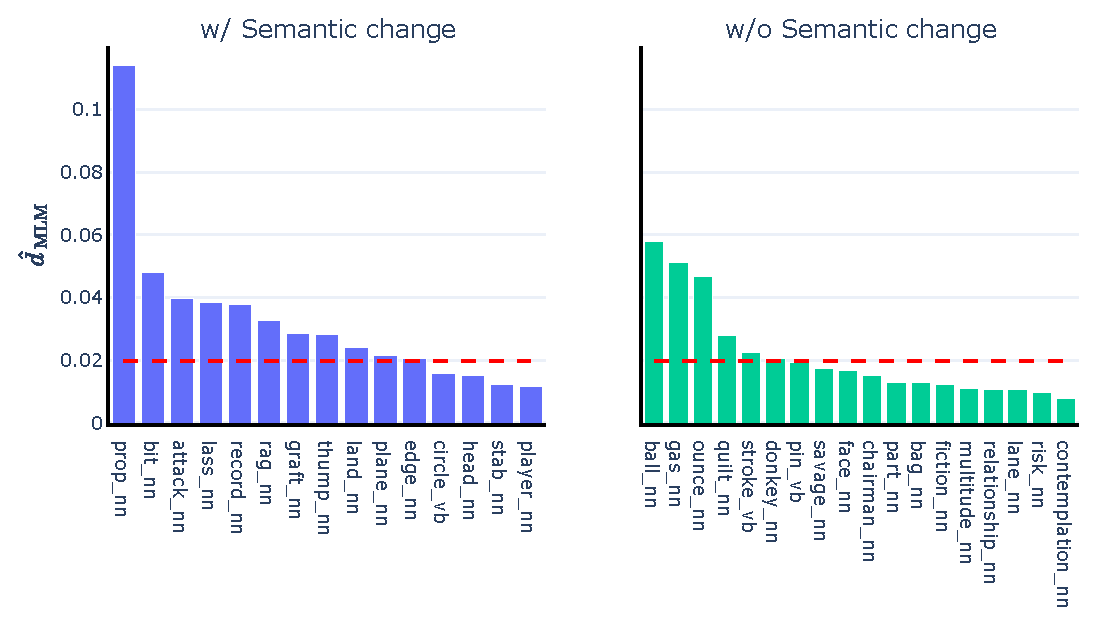
\includegraphics[width=0.8\textwidth]{../project/src/scale_5000-recursion_depth_10000/influences_binary.pdf}
\caption{\textbf{Predicted Influences.} The red dash lines are the threshold for binary classification.}
\label{fig:binary}
\end{figure*}


\begin{align}
\begin{split}
    &-\Delta L_\text{MLM}(\hat{\theta}, \hat{\theta}_{\setminus 1, t}) = \frac{-\mathcal{I}_\text{up, loss}(C_{\setminus 1, t}, C_\text{val})}{|C_1, C_2|} \\ 
    &-\Delta L_\text{MLM}(\hat{\theta}, \hat{\theta}_{\setminus 2, t}) = \frac{-\mathcal{I}_\text{up, loss}(C_{\setminus 2, t}, C_\text{val})}{|C_1, C_2|}    
    \label{eq:influence_fn_mlm}
\end{split}
\end{align}


As mentioned in Sec.~\ref{sec:background}, instead of forming and inverting the Hessian, I use the estimator developed in~\cite{second-order-approx} to approximate inverse hessian vector product: $H^{-1}_{\hat{\theta}} \nabla_\theta L_\text{MLM}(C_{\setminus 1, t}, \hat{\theta})$ and $H^{-1}_{\hat{\theta}} \nabla_\theta L_\text{MLM}(C_{\setminus 2, t}, \hat{\theta})$.

